% Vorlesung vom 17.12.2015
\renewcommand{\ldate}{2015-12-17}
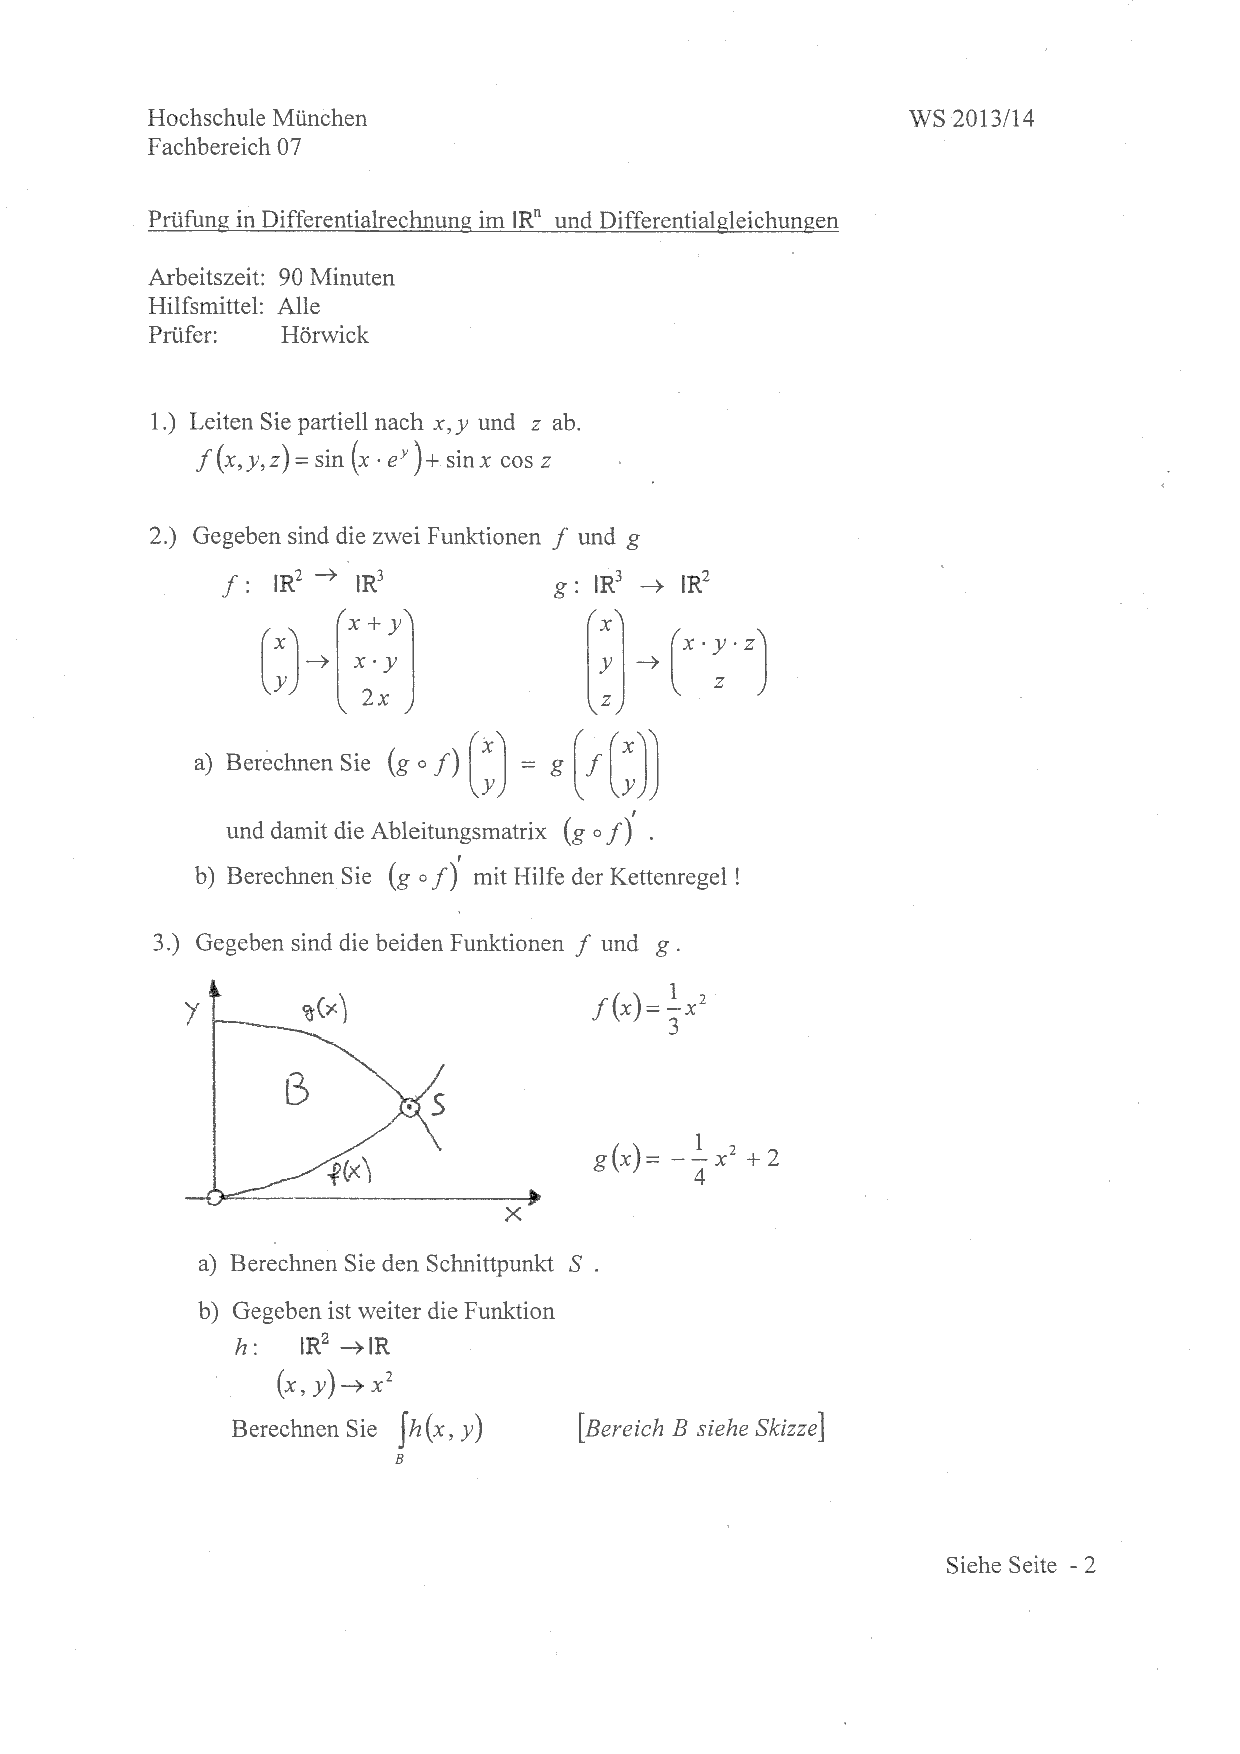
\includepdf[pages=-]{pruefungsangabe_ws1314}

\section{Lösung für die Prüfung WS 2013/14}

\subsection{zu 1)}
$f(x,y,z)$
$=\sin(x\cdot e^y) + \sin x \cos z$

$\frac{\df}{\dx} = \cos (x\cdot e^y) e^y + \cos x \cos z$

$\frac{\df}{\dy} = \cos (x\cdot e^y) x e^y $

$\frac{\df}{\dz} = -\sin x \sin z$

\subsection{zu 2a)}
$ (g\circ f) \vektor{x\\y} $
$= g\vektor{x+y\\x\cdot y\\2x}$
$=\vektor{(x+y) x y 2 x \\ 2x}$
$=\vektor{2x^3y + 2x^2y^2\\2x}$

\textbf{Ableitungsmatrix:}
$ (g\circ f)' \vektor{x\\y} $
$=\vektor{6yx^2 + 4xy^2, 2x^3 + 4x^2y\\2, 0}$

\subsection{zu 2b)}
$f'\vektor{x\\y}$
$=\vektor{1,1\\y,x\\2,0}$

$g'\vektor{x\\y\\z}$
$=\vektor{yz, xz, xy\\0,0,1}$

$
(g\circ f)' \vektor{x\\y} 
=g' \rbr{f \vektor{x\\y}}  \cdot f'\vektor{x\\y}
=g'\vektor{x+y\\x\cdot y\\2x}  \cdot \vektor{1,1\\y,x\\2,0} 
=\vektor{2x^2y, 2x^2+2xy,x^2y+y^2x\\0,0,1} \cdot \vektor{1,1\\y,x\\2,0} 
=...=\vektor{6yx^2 + 4xy^2, 2x^3+4x^2y\\2,0}
$\profnote{Matrizenmultiplikation: Zeile mal Spalte!}

\subsection{zu 3a)}
$f(x) = g(x)$

$\frac{1}{3} x^2 = -\frac{1}{4} x^2 + 2$

$x=1.85 \Rightarrow y = f(1.85) = 1.14 \Rightarrow S(1.85, 1.14)$

\subsection{zu 3b)}
$
\int_{B} h(x,y) 
=\int_{0}^{1.85} \rbr{\int_{f(x)}^{g(x)} h(x,y) dy} dx
=\int_{0}^{1.85} \rbr{ \int_{\frac{1}{3} x^2}^{-\frac{1}{4} x^2 + 2} x^2 dy} dx
=\int_{0}^{1.85} \sbr{yx^2}_{y=\frac{1}{3} x^2}^{y=-\frac{1}{4} x^2 + 2} dx
=\int_{0}^{1.85} \rbr{\rbr{-\frac{1}{4} x^2 + 2} x^2 - \frac{1}{3} x^2 x^2} dx
=\int_{0}^{1.85} -\frac{1}{4} x^4 + 2x^2 - \frac{1}{3} x^4 dx
=\int_{0}^{1.85} -\frac{7}{12} x^4 + 2x^2 dx
=\sbr{-\frac{7}{12} \cdot \frac{1}{5} x^5 + 2\cdot \frac{1}{3} x^3}_0^{1.85} 
=-\frac{7}{60} \cdot 1.85^5 + \frac{2}{3} \cdot 1.85^3
=1.69
$